\documentclass[english]{article}
\usepackage[utf8]{inputenc}
\usepackage[T1]{fontenc}
\usepackage{afterpage}
\usepackage{graphicx}
\usepackage{tabularx}
\usepackage{geometry}
\usepackage{listings}
\usepackage{amsmath}
\usepackage{xcolor}
\usepackage{babel}
\usepackage{float}
\usepackage{multirow}
\usepackage{array}
\newcolumntype{C}{>{\centering\arraybackslash}m{2cm}}
% Add in specific class to use \subsubsubsection, \paragraph, \subparagraph
\usepackage{titlesec}
\titleclass{\subsubsubsection}{straight}[\subsection]
\newcounter{subsubsubsection}[subsubsection]
\renewcommand\thesubsubsubsection{\thesubsubsection.\arabic{subsubsubsection}}
\renewcommand\theparagraph{\thesubsubsubsection.\arabic{paragraph}} % optional; useful if paragraphs are to be numbered
\titleformat{\subsubsubsection}
  {\normalfont\normalsize\bfseries}{\thesubsubsubsection}{1em}{}
\titlespacing*{\subsubsubsection}
{0pt}{3.25ex plus 1ex minus .2ex}{1.5ex plus .2ex}
\makeatletter
\renewcommand\paragraph{\@startsection{paragraph}{5}{\z@}%
  {3.25ex \@plus1ex \@minus.2ex}%
  {-1em}%
  {\normalfont\normalsize\bfseries}}
\renewcommand\subparagraph{\@startsection{subparagraph}{6}{\parindent}%
  {3.25ex \@plus1ex \@minus .2ex}%
  {-1em}%
  {\normalfont\normalsize\bfseries}}
\def\toclevel@subsubsubsection{4}
\def\toclevel@paragraph{5}
\def\toclevel@paragraph{6}
\def\l@subsubsubsection{\@dottedtocline{4}{7em}{4em}}
\def\l@paragraph{\@dottedtocline{5}{10em}{5em}}
\def\l@subparagraph{\@dottedtocline{6}{14em}{6em}}
\makeatother
\setcounter{secnumdepth}{4}
\setcounter{tocdepth}{3}
\geometry{left=1.5in, right=1.5in, top=1in, bottom=1.25in}
\titleformat{\section}{\clearpage\normalfont\Large\bfseries}{\thesection}{1em}{}
\usepackage{hyperref}
\hypersetup{
    colorlinks=true,
    linkcolor=black,
    filecolor=magenta,      
    urlcolor=blue,
    pdfpagemode=FullScreen,
}

\lstdefinestyle{mystyle}{
    language=Python, % Specify the programming language
    basicstyle=\ttfamily, % Set the font style (typewriter font)
    keywordstyle=\color{blue}, % Define keywords color
    commentstyle=\color{green}, % Define comments color
    numbers=none, % Display line numbers
    numberstyle=\tiny\color{gray}, % Line number font style
    breaklines=true, % Enable line wrapping
    frame=single, % Add a frame around the code
    tabsize=4 % Set the tab size
}

\definecolor{gray}{rgb}{0.5,0.5,0.5}

\begin{document}

\begin{titlepage}
\centering

\vspace{4cm} 

\Huge

Üzleti Intelligencia

\vspace{2cm} 

\Large

Megerősítéses tanulás - beadandó feladatok

\vspace{0.5cm}

2023 % Dátum

\vspace{2cm} 

\normalsize

A feladatok 1-3 skálán vannak osztályozva nehézség szerint, ahol 1 a legkönnyebb és 3 a legnehezebb. A feladatok véletlenszerűen sorsolódtak ki. A feladatok beadása Coospace felületen történik, ahol csak egy linket kell beküldeni, ami a feladatot megvalósító Git tárhelyre mutat. Késő beadás nem lehetséges, a dátum beadásakor feltöltött anyagok fognak leosztályozásra kerülni. Minden további információ a tantárgyi útmutatóban és az órán elhangzottakban találhatóak. \par\medskip
\begin{large}
\textbf{Az elégséges jegy feltételen, hogy minden részfeladat legalább 60\%-os sikerességgel megoldásra kerüljön.}
\end{large}
\end{titlepage}

\newpage

\section{MDP}

Implementálja az alábbi $MDP(S,A,P,R,s_0,\gamma)$ Markov döntési folyamatot. Az állapotok valószínűsége tizedes törtekként szerepel, a jutalmak pedig $+$ és $-$ előjellel a kapcsolatokon. Használja az alábbi paramétereket: $s_0 = 0, \; \gamma=0.98$

\begin{center}
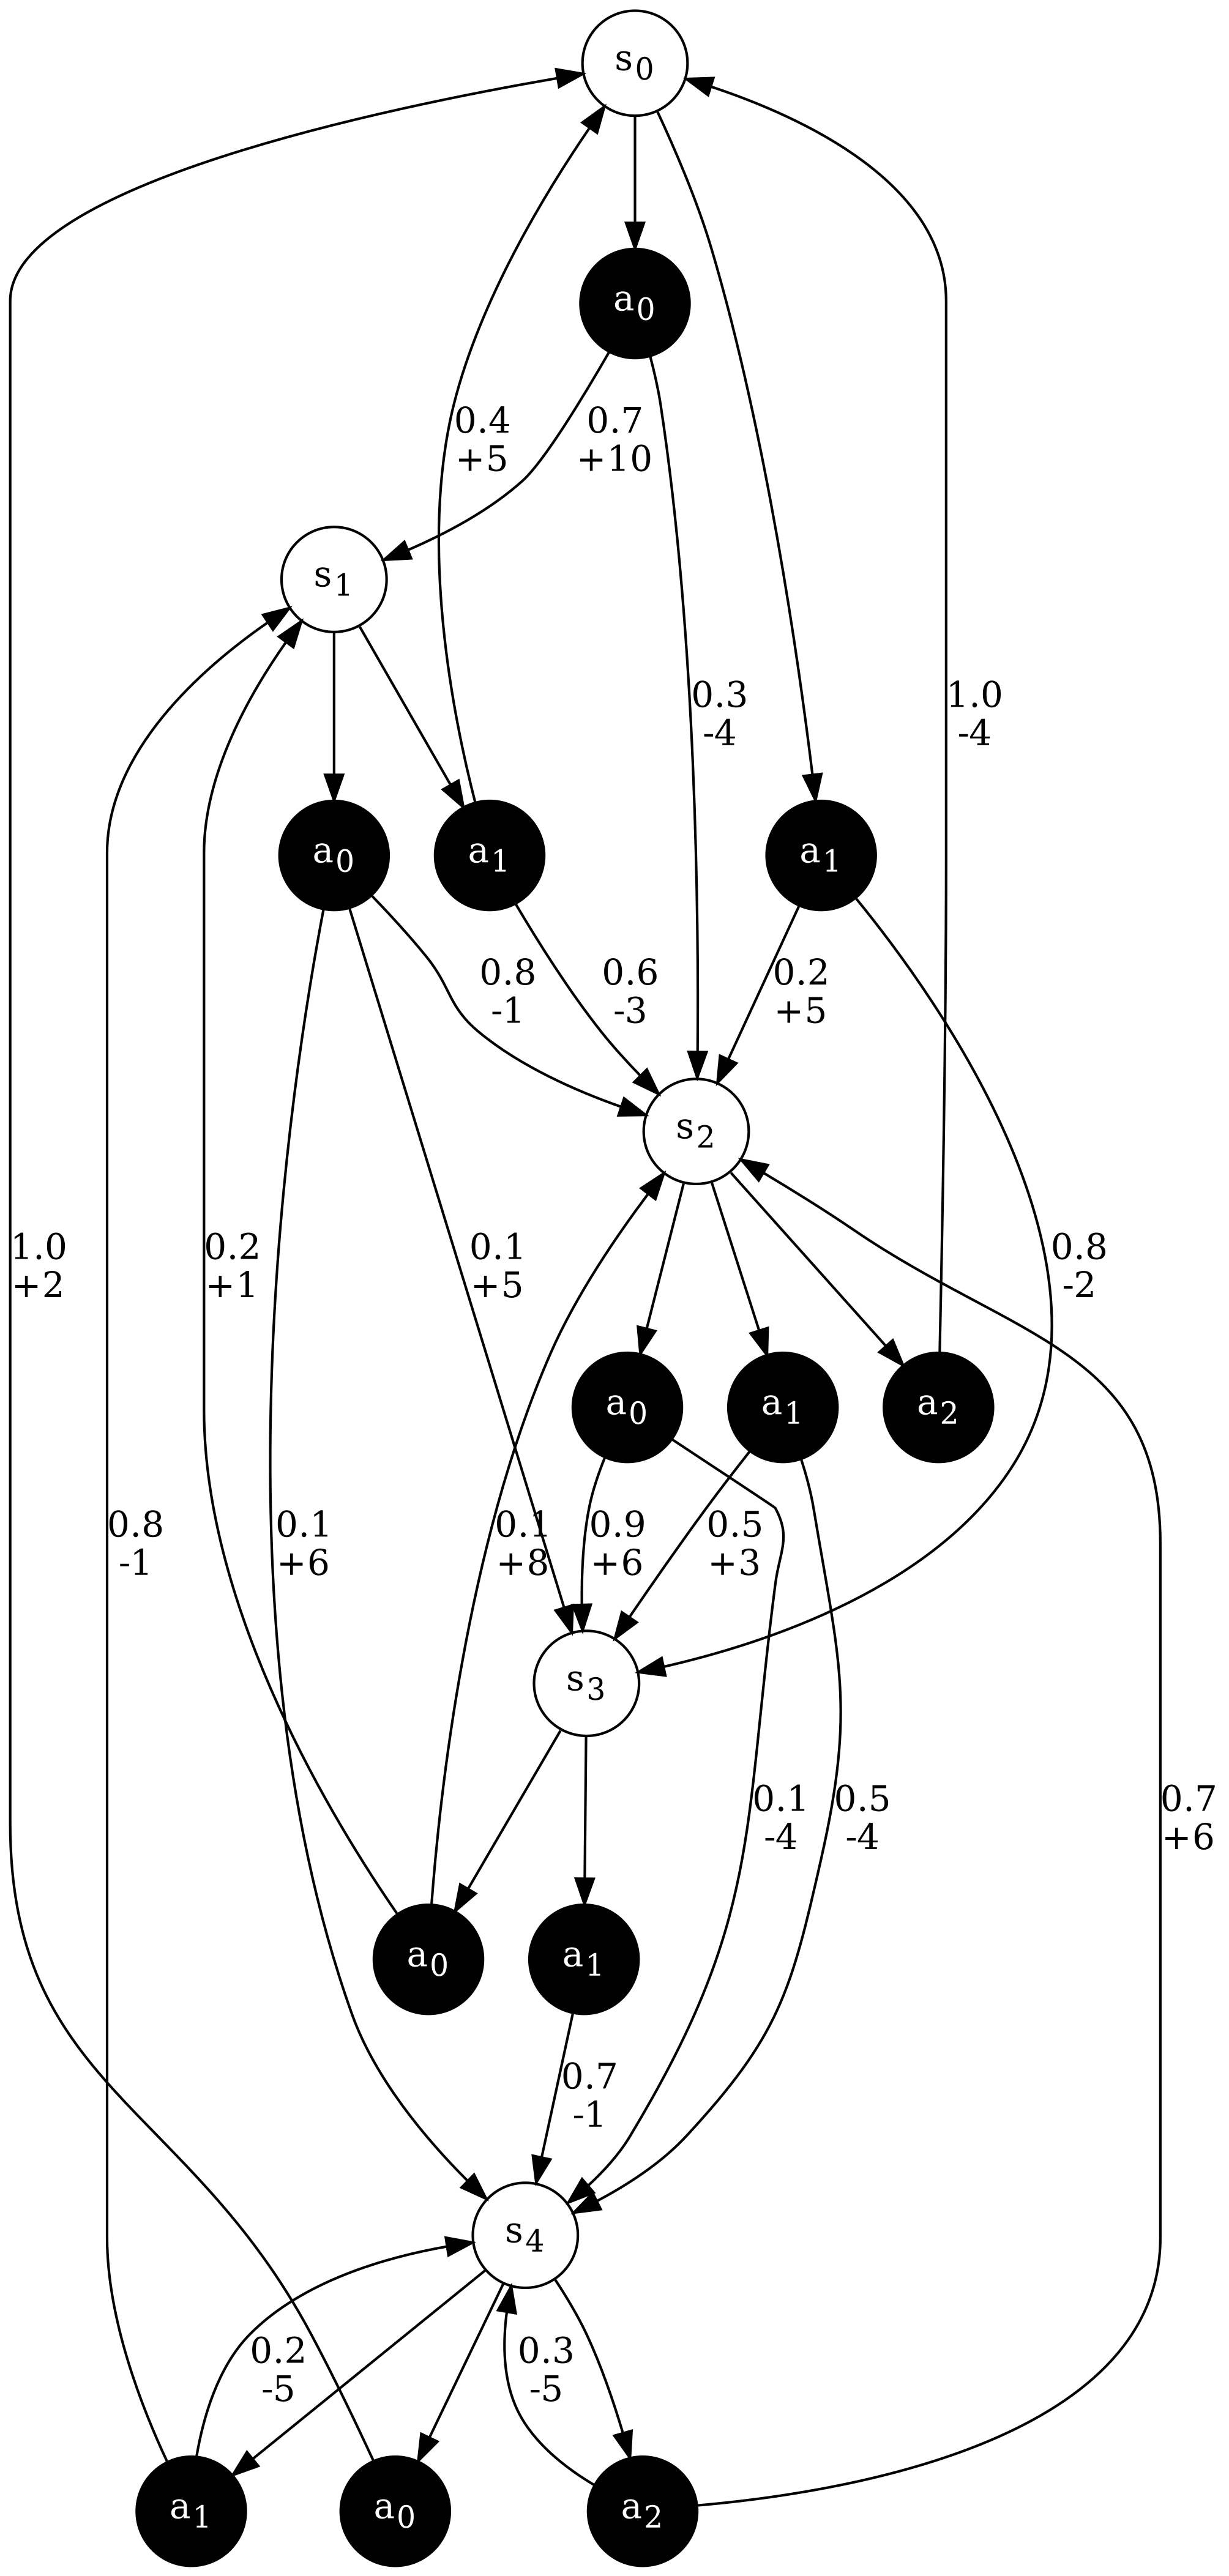
\includegraphics[width=\textwidth, height=19cm, keepaspectratio]{graphs/1_mdp.png}
\end{center}

\newpage{}

\subsection{(\textbf{A}) feladat}
\begin{itemize}
	\item Adja meg minden állapot értékét a megfelelő Bellman egyenlettel. Ábrázolja diagramon az értékek konvergenciáját.
	\item Adja meg z optimális politikát Monte Carlo algoritmussal. Ehhez tartozóan implementálja a MC politika keresés és kiértékelés algoritmusát. Ábrázolja diagramon az értékek konvergenciáját.
	\item Oldja meg a környezetet $Q$-tanulással. Adja meg az optimális politikát a $Q$-táblából származtatva. Ábrázolja a $Q$-értékek konvergenciáját diagramon. 
	\item Oldja meg a környezetet párbajozó mély Q-tanulással. Ábrázolja a jutalmak növekedését diagramon. 
	\item Minden feladatrészhez tartozóan írja le az eljárás elméleti alapjait és a saját tapasztalatait röviden egy Jupyter Markdown cellában.
\end{itemize}


\subsection{(\textbf{B}) feladat}
\begin{itemize}
	\item Oldja meg a környezetet dinamikus programozással. Ehhez tartozóan implementálja a politika iteráció algoritmusát. Adja meg az optimális politikát. Ábrázolja az értékek konvergenciáját diagramon.
	\item Adja meg az optimális politikát temporális különbségek algoritmusával. Ehhez tartozóan implementálja a TD politika keresés és kiértékelés algoritmusát. Ábrázolja diagramon az értékek konvergenciáját. 
	\item Oldja meg a környezetet dupla $Q$-tanulással. Adja meg az optimális politikát a dupla $Q$-táblából származtatottan. Ábrázolja az értékek konvergenciáját diagramon. 
	\item Oldja meg a környezetet dupla mély $Q$-tanulással. Ábrázolja a jutalmak növekedését diagramon. 
	\item Minden feladatrészhez tartozóan írja le az eljárás elméleti alapjait és a saját tapasztalatait röviden egy Jupyter Markdown cellában.
\end{itemize}


\end{document}
















